% !TeX spellcheck = cs_CZ
%{\tikzset{external/prefix={tikz/FYZII/}}
% \tikzset{external/figure name/.add={ch10_}{}}
%---------------------------------------------------------------------------------------------------
% file fey2ch10.tex
%---------------------------------------------------------------------------------------------------
%=========================== Kapitola: Dielektrika =================================================
\chapter{Dielektrika}\label{fyz:IIchaX}
\minitoc
  \section{Permitivita}\label{fyz:IIchaXsecI}
  \section{Vektor elektrické polarizace P}\label{fyz:IIchaXsecII}
  \section{Polarizační náboje}\label{fyz:IIchaXsecIII}
  \section{Elektrostatické rovnice pro dielektrika}\label{fyz:IIchaXsecIV}
  \section{Pole a síly v přítomnosti dielektrik}\label{fyz:IIchaXsecV}
  \section{Příklady a cvičení}\label{fyz:IIchaXsecVI}

    \begin{figure}[ht!] %\ref{fyz_fig705}
      \centering
      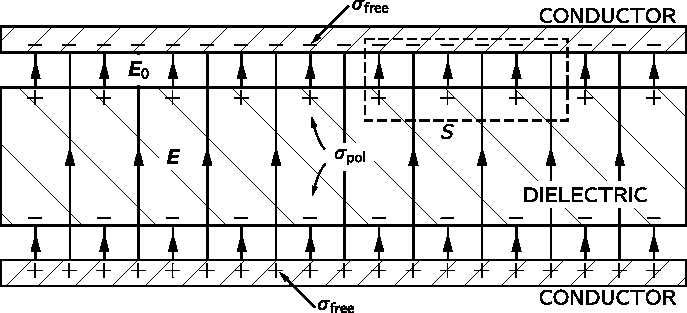
\includegraphics[width=0.9\linewidth]{fyz_fig705.pdf}
      \caption{
               (\cite[s.~707]{Feynman02})}
      \label{fyz_fig705}
    \end{figure}

    \begin{figure}[ht!] %\ref{fyz_fig706}
      \centering
      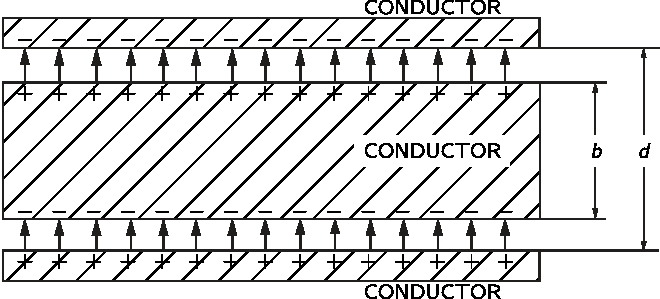
\includegraphics[width=0.9\linewidth]{fyz_fig706.pdf}
      \caption{
               (\cite[s.~707]{Feynman02})}
      \label{fyz_fig706}
    \end{figure}

    \begin{figure}[ht!] %\ref{fyz_fig707}
      \centering
      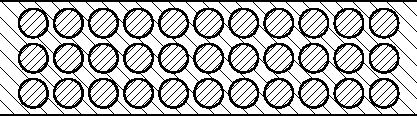
\includegraphics[width=0.9\linewidth]{fyz_fig707.pdf}
      \caption{
               (\cite[s.~707]{Feynman02})}
      \label{fyz_fig707}
    \end{figure}

    \begin{figure}[ht!]
      \centering
      \begin{tabular}{c}
        \subfloat[ ]{\label{fyz_fig708a}
          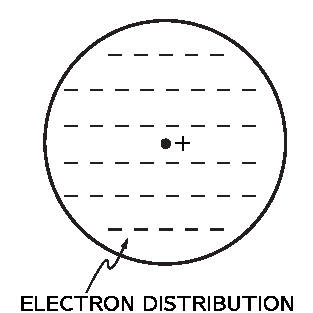
\includegraphics[width=0.6\linewidth]{fyz_fig708a.pdf}}               \\
        \subfloat[ ]{\label{fyz_fig708b}
          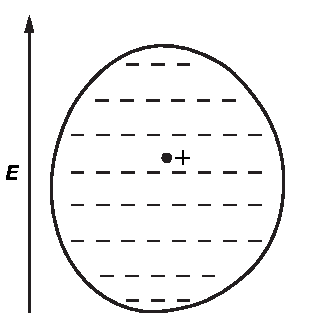
\includegraphics[width=0.6\linewidth]{fyz_fig708b.pdf}}
      \end{tabular}
      \label{fyz_fig708}
      \caption{
               (\cite[s.~748]{Feynman02})}
    \end{figure}

    \begin{figure}[ht!] %\ref{fyz_fig709}
      \centering
      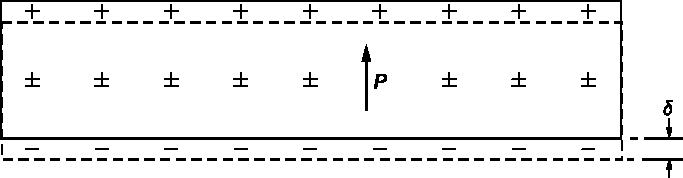
\includegraphics[width=0.7\linewidth]{fyz_fig709.pdf}
      \caption{
               (\cite[s.~707]{Feynman02})}
      \label{fyz_fig709}
    \end{figure}

    \begin{figure}[ht!] %\ref{fyz_fig710}
      \centering
      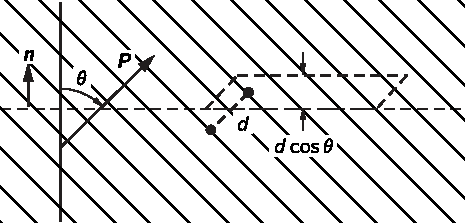
\includegraphics[width=0.7\linewidth]{fyz_fig710.pdf}
      \caption{
               (\cite[s.~707]{Feynman02})}
      \label{fyz_fig710}
    \end{figure}

    \begin{figure}[ht!] %\ref{fyz_fig711}
      \centering
      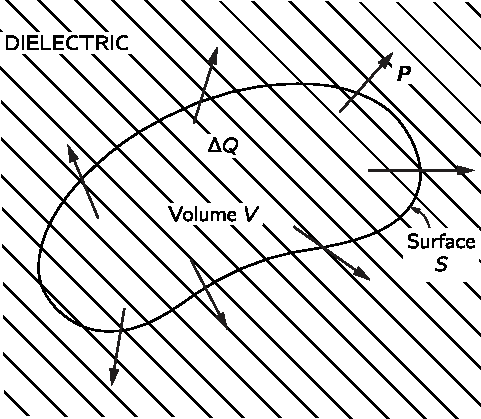
\includegraphics[width=0.7\linewidth]{fyz_fig711.pdf}
      \caption{
               (\cite[s.~707]{Feynman02})}
      \label{fyz_fig711}
    \end{figure}

    \begin{figure}[ht!] %\ref{fyz_fig712}
      \centering
      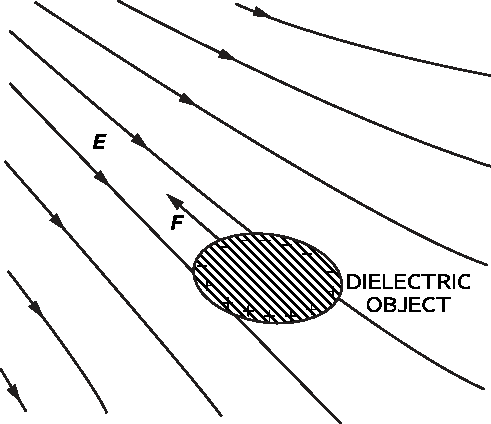
\includegraphics[width=0.7\linewidth]{fyz_fig712.pdf}
      \caption{
               (\cite[s.~707]{Feynman02})}
      \label{fyz_fig712}
    \end{figure}

    \begin{figure}[ht!] %\ref{fyz_fig713}
      \centering
      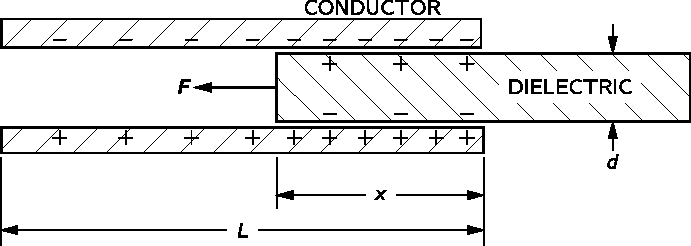
\includegraphics[width=0.7\linewidth]{fyz_fig713.pdf}
      \caption{
               (\cite[s.~707]{Feynman02})}
      \label{fyz_fig713}
    \end{figure}


%} %tikzset
%---------------------------------------------------------------------------------------------------
%\printbibliography[title={Seznam literatury},heading=subbibliography]
\addcontentsline{toc}{section}{Seznam literatury}